\documentclass{article}
\usepackage{geometry}
\geometry{margin=0.5cm, paperheight=50cm, paperwidth=21cm}
\usepackage{tikz}
\usetikzlibrary{shapes.geometric, arrows.meta, positioning, calc}
\usepackage{amssymb}

\begin{document}

\begin{center}
\Large\bfseries
Execution Flow Visualization
\end{center}

\section*{Program Execution Flowchart}

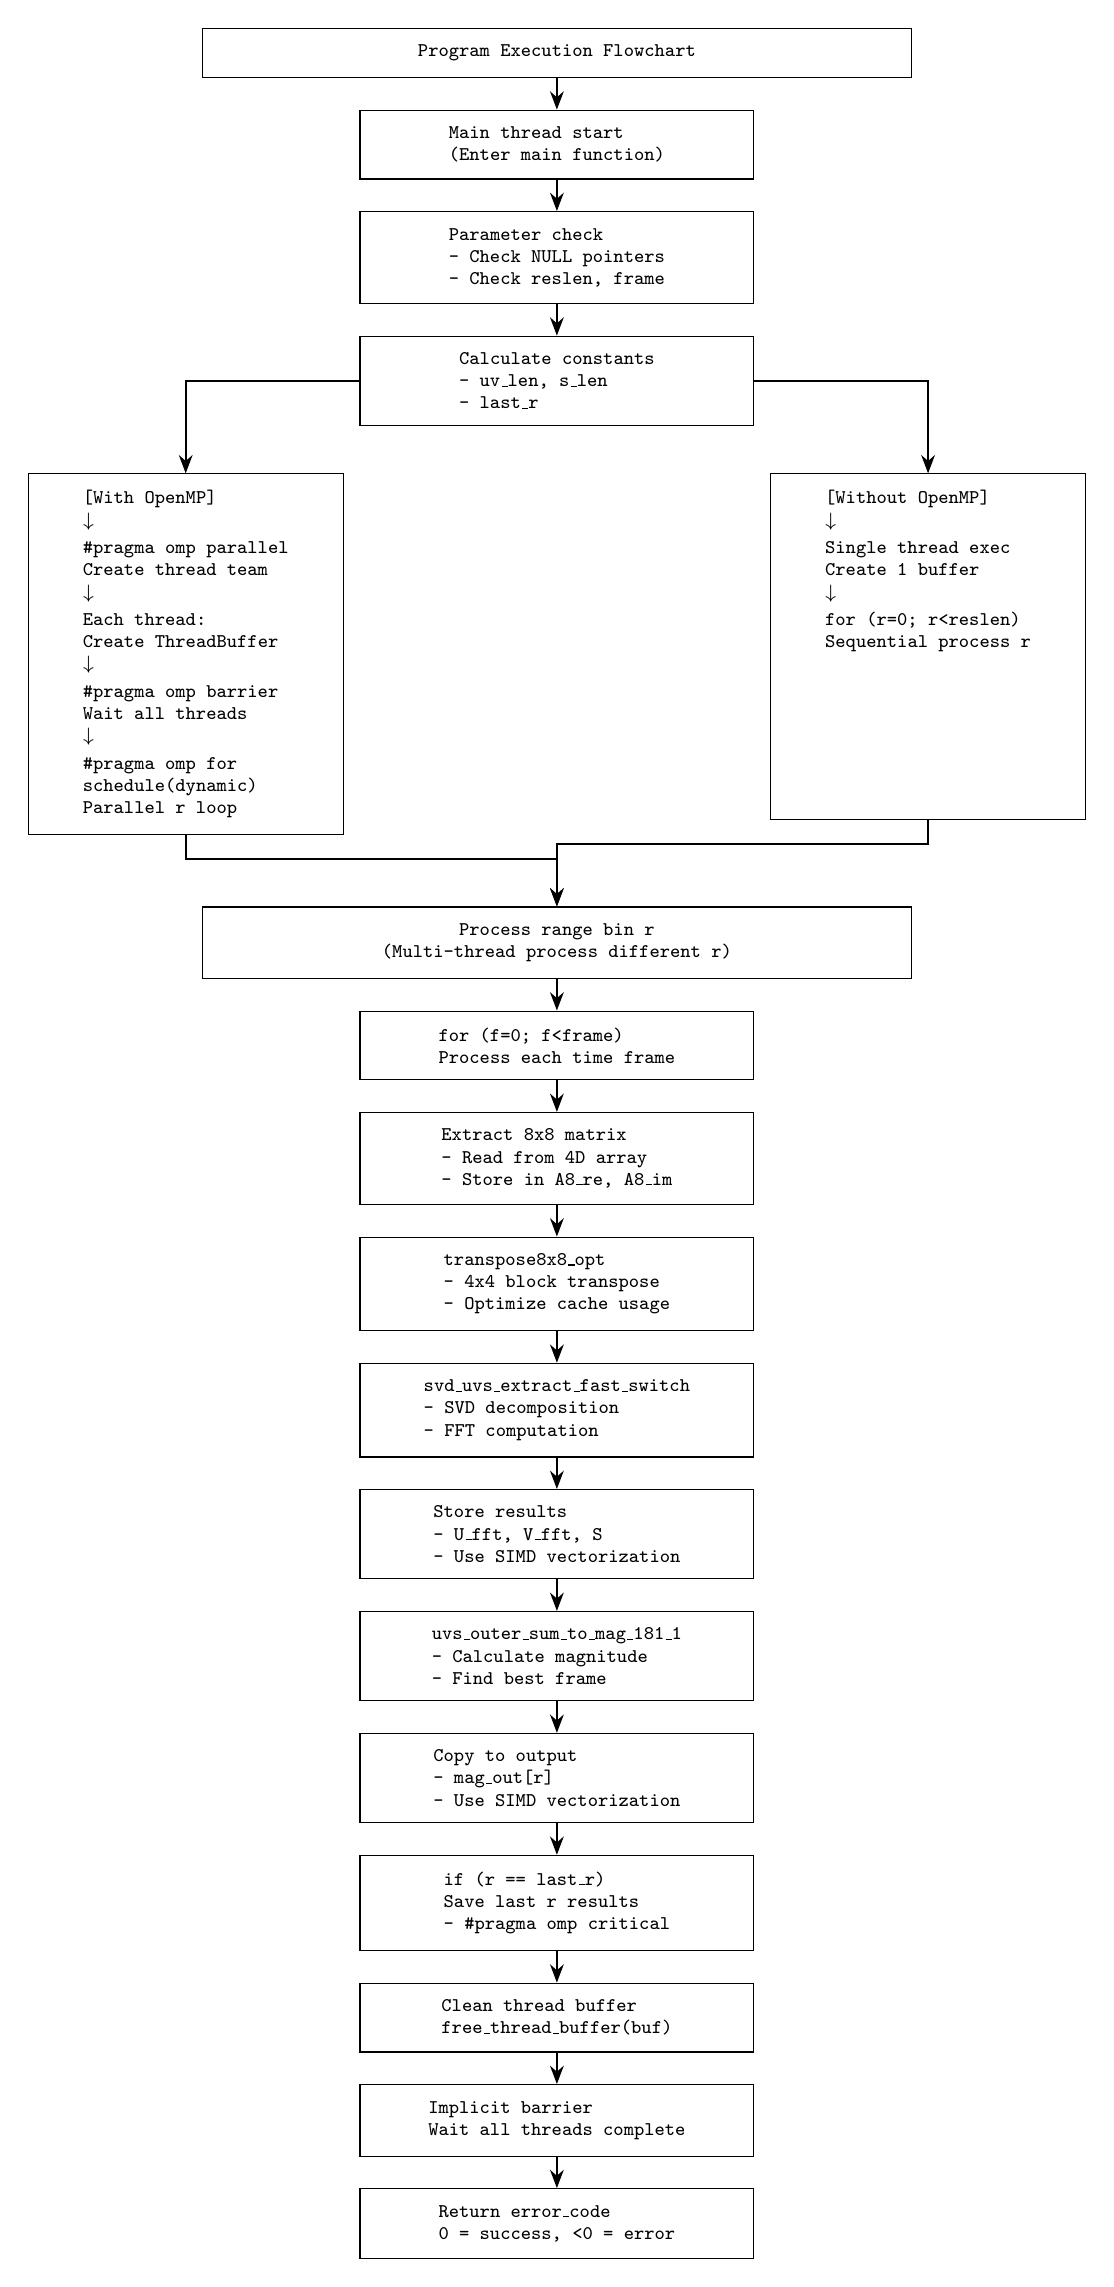
\begin{tikzpicture}[
    node distance=0.4cm,
    box/.style={draw, rectangle, minimum width=5cm, align=left, font=\ttfamily\scriptsize, inner sep=6pt},
    widebox/.style={draw, rectangle, minimum width=9cm, align=center, font=\ttfamily\scriptsize, inner sep=6pt},
    smallbox/.style={draw, rectangle, minimum width=4cm, align=left, font=\ttfamily\scriptsize, inner sep=6pt},
    arrow/.style={->, >=Stealth, thick}
]

% Title box
\node[widebox] (title) {Program Execution Flowchart};

% Main flow
\node[box, below=of title] (start) {Main thread start\\(Enter main function)};
\node[box, below=of start] (param) {Parameter check\\- Check NULL pointers\\- Check reslen, frame};
\node[box, below=of param] (calc) {Calculate constants\\- uv\_len, s\_len\\- last\_r};

% Parallel boxes
\node[smallbox, below left=0.6cm and 0.2cm of calc] (omp) {[With OpenMP]\\$\downarrow$\\[2pt]\#pragma omp parallel\\Create thread team\\$\downarrow$\\[2pt]Each thread:\\Create ThreadBuffer\\$\downarrow$\\[2pt]\#pragma omp barrier\\Wait all threads\\$\downarrow$\\[2pt]\#pragma omp for\\schedule(dynamic)\\Parallel r loop};

\node[smallbox, below right=0.6cm and 0.2cm of calc] (noomp) {[Without OpenMP]\\$\downarrow$\\[2pt]Single thread exec\\Create 1 buffer\\$\downarrow$\\[2pt]for (r=0; r<reslen)\\Sequential process r\\~\\~\\~\\~\\~\\~\\~};

% Merge point
\coordinate (merge) at ($(omp.south)!0.5!(noomp.south) + (0,-1cm)$);
\node[widebox, anchor=north] (process) at (merge) {Process range bin r\\(Multi-thread process different r)};

\node[box, below=of process] (forloop) {for (f=0; f<frame)\\Process each time frame};

\node[box, below=of forloop] (extract) {Extract 8x8 matrix\\- Read from 4D array\\- Store in A8\_re, A8\_im};

\node[box, below=of extract] (transpose) {transpose8x8\_opt\\- 4x4 block transpose\\- Optimize cache usage};

\node[box, below=of transpose] (svd) {svd\_uvs\_extract\_fast\_switch\\- SVD decomposition\\- FFT computation};

\node[box, below=of svd] (store) {Store results\\- U\_fft, V\_fft, S\\- Use SIMD vectorization};

\node[box, below=of store] (mag) {uvs\_outer\_sum\_to\_mag\_181\_1\\- Calculate magnitude\\- Find best frame};

\node[box, below=of mag] (copy) {Copy to output\\- mag\_out[r]\\- Use SIMD vectorization};

\node[box, below=of copy] (lastr) {if (r == last\_r)\\Save last r results\\- \#pragma omp critical};

\node[box, below=of lastr] (clean) {Clean thread buffer\\free\_thread\_buffer(buf)};

\node[box, below=of clean] (barrier) {Implicit barrier\\Wait all threads complete};

\node[box, below=of barrier] (return) {Return error\_code\\0 = success, <0 = error};

% Arrows for main flow
\draw[arrow] (title) -- (start);
\draw[arrow] (start) -- (param);
\draw[arrow] (param) -- (calc);
\draw[arrow] (calc) -| (omp);
\draw[arrow] (calc) -| (noomp);
\draw[arrow] (omp.south) -- ++(0,-0.3cm) -| (process.north);
\draw[arrow] (noomp.south) -- ++(0,-0.3cm) -| (process.north);
\draw[arrow] (process) -- (forloop);
\draw[arrow] (forloop) -- (extract);
\draw[arrow] (extract) -- (transpose);
\draw[arrow] (transpose) -- (svd);
\draw[arrow] (svd) -- (store);
\draw[arrow] (store) -- (mag);
\draw[arrow] (mag) -- (copy);
\draw[arrow] (copy) -- (lastr);
\draw[arrow] (lastr) -- (clean);
\draw[arrow] (clean) -- (barrier);
\draw[arrow] (barrier) -- (return);

\end{tikzpicture}

\vspace{1cm}

\section*{Multi-thread Execution Timeline}

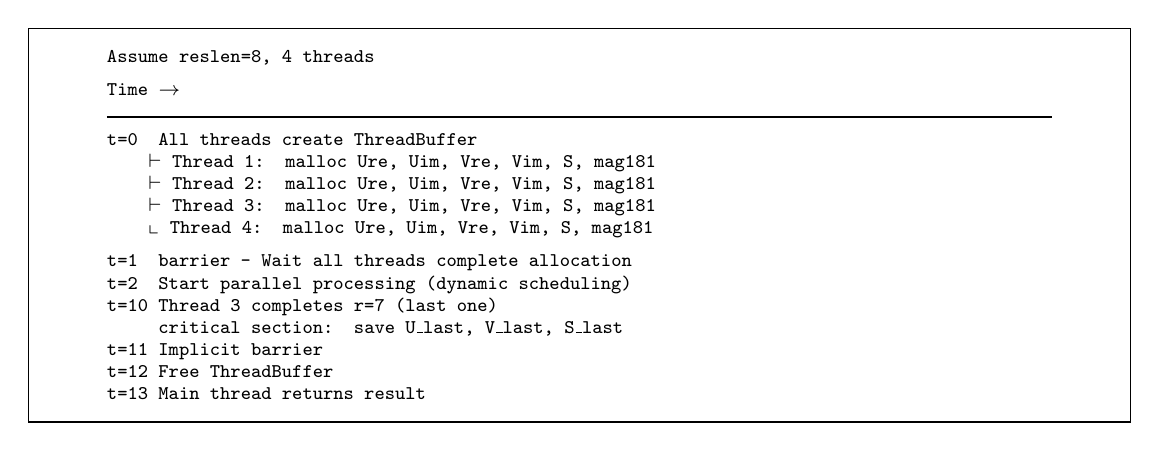
\begin{tikzpicture}[
    node distance=0.3cm,
    timeline/.style={draw, rectangle, minimum width=14cm, align=left, font=\ttfamily\scriptsize, inner sep=8pt}
]

\node[timeline] (tl) {
Assume reslen=8, 4 threads\\[4pt]
Time $\rightarrow$\\
\rule{12cm}{0.5pt}\\[2pt]
t=0~~All threads create ThreadBuffer\\
~~~~$\vdash$ Thread 1: malloc Ure, Uim, Vre, Vim, S, mag181\\
~~~~$\vdash$ Thread 2: malloc Ure, Uim, Vre, Vim, S, mag181\\
~~~~$\vdash$ Thread 3: malloc Ure, Uim, Vre, Vim, S, mag181\\
~~~~$\llcorner$ Thread 4: malloc Ure, Uim, Vre, Vim, S, mag181\\[4pt]
t=1~~barrier - Wait all threads complete allocation\\
t=2~~Start parallel processing (dynamic scheduling)\\
t=10 Thread 3 completes r=7 (last one)\\
~~~~~critical section: save U\_last, V\_last, S\_last\\
t=11 Implicit barrier\\
t=12 Free ThreadBuffer\\
t=13 Main thread returns result
};

\end{tikzpicture}

\end{document}